
\documentclass[letterpaper,11pt]{article}
\usepackage{latexsym}
\usepackage[empty]{fullpage}
\usepackage[usenames,dvipsnames]{color}
\usepackage{verbatim}
\usepackage{hyperref}
\usepackage{framed}
\usepackage{tocloft}
\usepackage{bibentry}
\usepackage{amsmath}
\usepackage{scrextend}
\usepackage{listings}
\usepackage{color}
\usepackage{fancyhdr}
\usepackage{graphicx}
\usepackage{pgfplots}
% Adjust margins
\usepackage[left=1in,top=0.7in,right=1in,bottom=0.6in]{geometry}

  %THIS PORTION IS FOR ADDING PAGE NUMBER
  \pagestyle{fancy}
  \cfoot{}
  \rfoot{\thepage}
  \renewcommand{\headrulewidth}{0pt}
  %THIS PORTION IS FOR ADDING PAGE NUMBER.


  \urlstyle{same}
  \definecolor{mygrey}{gray}{.85}
  \definecolor{mygreylink}{gray}{.30}
  \textheight=9.0in
  \raggedbottom
  \raggedright
  \setlength{\tabcolsep}{0in}


  %The following part is for inserting codes in LaTeX:
  \definecolor{codegreen}{rgb}{0,0.6,0}
  \definecolor{codegray}{rgb}{0.5,0.5,0.5}
  \definecolor{codepurple}{rgb}{0.58,0,0.82}
  \definecolor{backcolour}{rgb}{0.95,0.95,0.92}

  \lstdefinestyle{mystyle}{
      backgroundcolor=\color{backcolour},
      commentstyle=\color{codegreen},
      keywordstyle=\color{magenta},
      numberstyle=\tiny\color{codegray},
      stringstyle=\color{codepurple},
      basicstyle=\footnotesize,
      breakatwhitespace=false,
      breaklines=true,
      captionpos=b,
      keepspaces=true,
      numbers=left,
      numbersep=5pt,
      showspaces=false,
      showstringspaces=false,
      showtabs=false,
      tabsize=2
  }
  \lstset{style=mystyle}
  %For inserting codes in LaTeX

  \begin{document}

  \begin{center}
  	\textbf{\Huge{Advanced Data Analysis HW2}}
  \end{center}

  \begin{center}
  	\textsl{Ao Liu, al3472}
  \end{center}


  \bigbreak
  \bigbreak
  \bigbreak

  %%%%%%%%%%%%%%%%%%%%%%%%%%%%%%%%%%%%%
  %%%%%%%%%%%%%%   1   %%%%%%%%%%%%%%%%
  %%%%%%%%%%%%%%%%%%%%%%%%%%%%%%%%%%%%%


\begin{addmargin}[-2em]{0em}
\large{\textbf{1. }}\end{addmargin}
\begin{addmargin}[-1.1em]{0em} \textbf{Suppose you have three different feeds that may affect the size of eggs that chickens lay. You randomly assign 10 chickens to each one of the three feeds and record the size of the eggs (maximum length, in centimeters) that the chickens lay the following week. The null hypothesis is that all the chicken feeds have the same effect on the length of the major axis. The alternative is that the feed has some causal effect. A partial output is}\par \end{addmargin}


\begin{center}
\begin{tabular}{ p{2cm}p{1cm}p{1cm}p{1cm}p{1cm}}
\centering Source & df & SS & MS & F\\
\centering feed & {} & 23.43 & {} & {}\\
\centering error & {} & {} & {} & {}\\
\centering total & {} & 28.10 & {} & {}\\
\end{tabular}
\end{center}


\begin{addmargin}[-1.1em]{0em} \textbf{(a)  Complete the table above}\par \end{addmargin}

\bigbreak
\begin{addmargin}[-0.5em]{0em}
\textbf{Answer: }\end{addmargin}

\begin{center}
\begin{tabular}{ p{2cm}p{1.5cm}p{1.5cm}p{1.5cm}p{1.5cm}}
\centering Source & df & SS & MS & F\\
\centering feed & 2 & 23.43 & 11.715 & 67.731\\
\centering error & 27 & 4.67 & 0.1730 & {}\\
\centering total & 29 & 28.10 & {} & {}\\
\end{tabular}
\end{center}

\begin{addmargin}[-1.1em]{0em}
\textbf{(b)}\par\end{addmargin}
  \textbf{Test the null hypothesis that all the chicken feeds have the same effect on the length of the major axis against the alternative that the feed has some causal effect. Use $\alpha = 0.05$.
}\par
\bigbreak

\begin{addmargin}[-0.5em]{0em}
\textbf{Answer: }\end{addmargin}

\begin{lstlisting}
>qf(.95, df1=2, df2=27)
[1] 3.354131
\end{lstlisting}

Since $F = 67.731 > F(0.95, 2, 29) = 3.354131$, we reject the null hypothesis that all the chicken feeds have the same effect.



%%%%%%%%%%%%%%%%%%%%%%%%%%%%%%%%%%%%%
%%%%%%%%%%%%%%   2   %%%%%%%%%%%%%%%%
%%%%%%%%%%%%%%%%%%%%%%%%%%%%%%%%%%%%%


  \begin{addmargin}[-2em]{0em} \large{\textbf{2. }}\end{addmargin}

  \begin{addmargin}[-1.1em]{0em} \textbf{Suppose you want to compare the types of popcorn popper and the brand of popcorn with respect to their yield (in terms of cups of popped corn). Factor A is the type of popper: oil-based versus air-based. Factor B is the brand of popcorn: gourmet versus national brand versus generic. For each combination of popper type and brand, you took three separate measurements. The ANOVA table is}\par\end{addmargin}

    \begin{center}
    \begin{tabular}{ p{5cm}p{1cm}p{1cm}p{1cm}p{1cm}}
    \centering Source & df & SS & MS & F\\
    \centering Propper(A) & {} & 4.5 & {} &\\
    \centering Corn(B) & {} & 15.75 & {} & {}\\
    \centering Interaction (A*B) & {} & {} & {} & {}\\
    \centering error & {} & 1.67 & {} & {}\\
    \centering total & {} & 22.00 & {} & {}\\
    \end{tabular}
    \end{center}

  \bigbreak

  \begin{addmargin}[-1.1em]{0em}
  \textbf{(a)}\par\end{addmargin}
    \textbf{Complete the table above.}\par
  \bigbreak
  \begin{addmargin}[-0.5em]{0em}
  \textbf{Answer: }\end{addmargin}

  \begin{center}
  \begin{tabular}{ p{5cm}p{1cm}p{1.5cm}p{1.5cm}p{1.5cm}}
  \centering Source & df & SS & MS & F\\
  \centering Propper(A) & 1 & 4.5 & 4.5 & 32.374\\
  \centering Corn(B) & 2 & 15.75 & 7.875 & 56.655\\
  \centering Interaction (A*B) & 2 & 0.08 & 0.04 & 0.2878\\
  \centering error & 12 & 1.67 & 0.139 & {}\\
  \centering total & 17 & 22.00 & 1.294 & {}\\
  \end{tabular}
  \end{center}


  \bigbreak
  \begin{addmargin}[-1.1em]{0em}
  \textbf{(b)}\par\end{addmargin}
    \textbf{Test $H_0$ : No interaction against H1 : there is an interaction, use $\alpha = 0.05$.}\par
  \bigbreak
  \begin{addmargin}[-0.5em]{0em}
  \textbf{Answer: }\end{addmargin}


\begin{lstlisting}
>qf(.95, df1=2, df2=12)
[1] 3.885294
\end{lstlisting}
Since $F = 32.374 > F(0.95,1,12) = 3.885294$, we rejuct the null hypothesis that there is no interaciton.

  \bigbreak
  \begin{addmargin}[-1.1em]{0em}
  \textbf{(c)}\par\end{addmargin}
    \textbf{It is decided to fit a model without an interaction and the partial results are}\par

    \begin{center}
    \begin{tabular}{ p{5cm}p{1cm}p{1cm}p{1cm}p{1cm}}
    \centering Source & df & SS & MS & F\\
    \centering Propper(A) & {} & 4.5 & {} &\\
    \centering Corn(B) & {} & 15.75 & {} & {}\\
    \centering error & {} & 1.67 & {} & {}\\
    \centering total & {} & 22.00 & {} & {}\\
    \end{tabular}
    \end{center}

  \begin{addmargin}[-0.5em]{0em}
  \textbf{Answer: }\end{addmargin}

  \bigbreak
  \begin{addmargin}[-1.1em]{0em}
  \textbf{(d)}\par\end{addmargin}
    \textbf{Complete the table above.}\par
  \bigbreak
  \begin{addmargin}[-0.5em]{0em}
  \textbf{Answer: }\end{addmargin}

  \begin{center}
  \begin{tabular}{ p{5cm}p{1cm}p{1.5cm}p{1.5cm}p{1.5cm}}
  \centering Source & df & SS & MS & F\\
  \centering Propper(A) & 1 & 4.5 & 4.5 & 37.72\\
  \centering Corn(B) & 2 & 15.75 & 7.875 & 66.01\\
  \centering error & 14 & 1.67 & 0.1193 & {}\\
  \centering total & 17 & 22.00 & {} & {}\\
  \end{tabular}
  \end{center}

  \bigbreak
  \begin{addmargin}[-1.1em]{0em}
  \textbf{(e)}\par\end{addmargin}
    \textbf{Test $H_0$: No popper effect against $H_1$: there is a popper effect. Use $\alpha = 0.05$}\par
  \bigbreak
  \begin{addmargin}[-0.5em]{0em}
  \textbf{Answer: }\end{addmargin}

\begin{lstlisting}
>qf(.95, df1=1, df2=14)
[1] 4.60011
\end{lstlisting}
Since $F = 37.72 > F(0.95,1,14) = 4.6001$, we reject the null hypothesis that there is no popper effect


    \bigbreak
    \begin{addmargin}[-1.1em]{0em}
    \textbf{(f)}\par\end{addmargin}
      \textbf{Test $H_0$: No corn effect against $H_1$ : there is a corn effect. Use $\alpha = 0.05$.
}\par
    \bigbreak
    \begin{addmargin}[-0.5em]{0em}
    \textbf{Answer: }\end{addmargin}


\begin{lstlisting}
>qf(.95, df1=2, df2=14)
[1] 3.738892
\end{lstlisting}
Since $F = 66.01 > F(0.95,2,14) = 3.738892$, we reject the null hypothesis that there is no corn effect


  %%%%%%%%%%%%%%%%%%%%%%%%%%%%%%%%%%%%%
  %%%%%%%%%%%%%%   3   %%%%%%%%%%%%%%%%
  %%%%%%%%%%%%%%%%%%%%%%%%%%%%%%%%%%%%%

  \bigbreak
  \begin{addmargin}[-2em]{0em} \large{\textbf{3. }}\end{addmargin}

  \begin{addmargin}[-1.1em]{0em} \textbf{In this exercise A and B are two fertilizers types, M, N, O and P are four wheat types and yijk values are wheat yields in bushels per plot (one third of an acre) corresponding to the different combinations of fertilizer type and wheat type. Also, assume that this data was obtained by using a completely randomized experimental design. (see HW2data.csv)
}\par\end{addmargin}
  \end{addmargin}

    \bigbreak
    \begin{addmargin}[-1.1em]{0em}
    \textbf{(a)}\par\end{addmargin}
      \textbf{Construct an interaction plot? Does it suggest that there is an interaction between fertilizer type and wheat type?}\par
    \bigbreak
    \begin{addmargin}[-0.5em]{0em}
    \textbf{Answer:}\end{addmargin}

\begin{lstlisting}
>data <- read.csv("HW2DATA.csv")
>fertilizer <- c(rep("A",12),rep("B",12))
>wheat <- data[,2]
>response <- data[,3]
>interaction.plot(fertilizer,wheat,response)
\end{lstlisting}

we get the following interaction plot:

\begin{center}
\makebox[\linewidth]{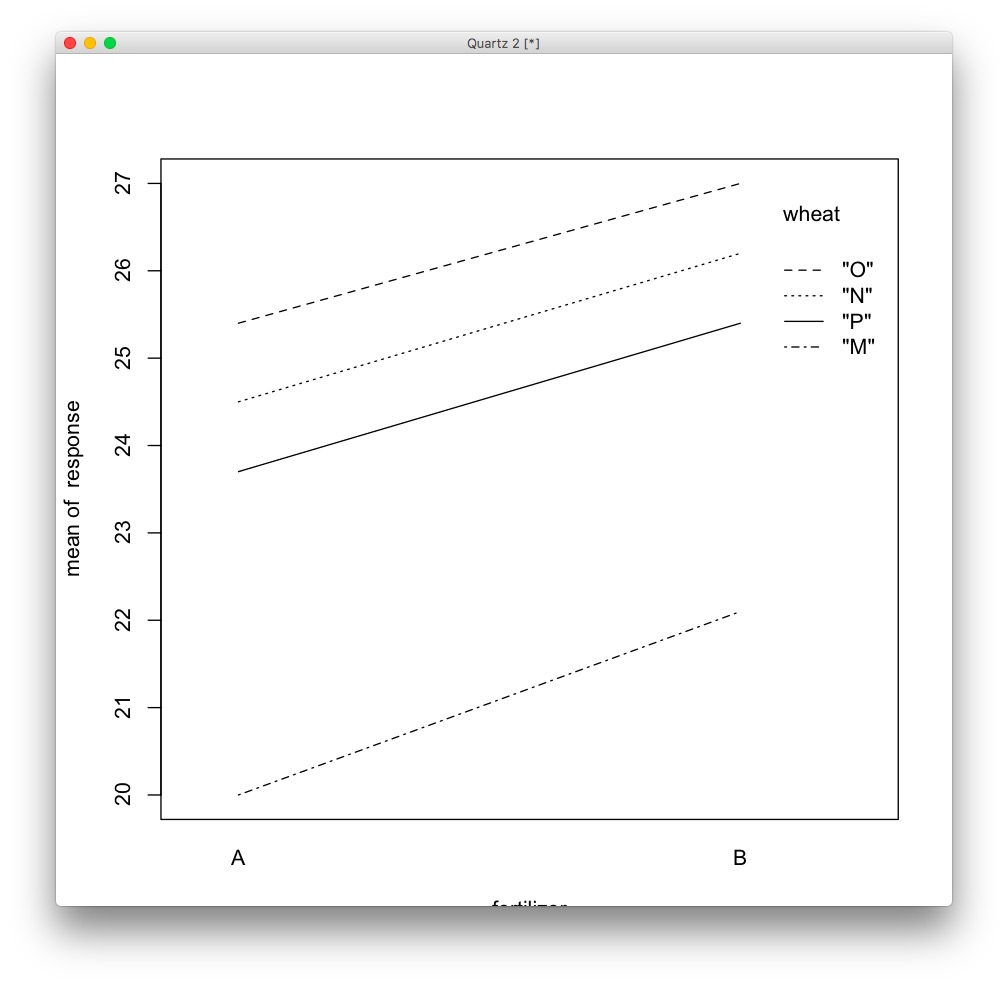
\includegraphics[width=\textwidth]{HW21.jpg}}
\end{center}

The four lines are parallel to each other, suggesting that the there is no interaction between fertilizer type and wheat type.

    \bigbreak
    \begin{addmargin}[-1.1em]{0em}
    \textbf{(b)}\par\end{addmargin}
      \textbf{Test $H_0$ : No interaction against $H_1$ : there is an interaction, use $\alpha = 0.05$.}\par
    \bigbreak
    \begin{addmargin}[-0.5em]{0em}
    \textbf{Answer: }\end{addmargin}


\begin{lstlisting}
>summary(aov(response~fertilizer*wheat))
\end{lstlisting}
  we get the following result:

\begin{lstlisting}
                 Df Sum Sq Mean Sq F value   Pr(>F)
fertilizer        1  18.90  18.904   48.63 3.14e-06 ***
wheat             3  92.02  30.674   78.90 8.37e-10 ***
fertilizer:wheat  3   0.22   0.074    0.19    0.902
Residuals        16   6.22   0.389
---
Signif. codes:  0 '***' 0.001 '**' 0.01 '*' 0.05 '.' 0.1 ' ' 1
\end{lstlisting}

Since the p-value for "fertilizer:wheat" is $0.902>\alpha = 0.05$, then we cannot reject $H_0$.

\bigbreak
\begin{addmargin}[-1.1em]{0em}
\textbf{(c)}\par\end{addmargin}
\textbf{Fit a model without an interaction and test $H_0$: No fertilizer effect against $H_1$ : there is a fertilizer effect. Use $\alpha = 0.05$ if you reject $H_0$, use Tukey’s method to do pairwise comparisons of the different fertilizer types.}\par
    \bigbreak
    \begin{addmargin}[-0.5em]{0em}    \textbf{Answer: }\end{addmargin}
We fit a model without interaction:
\begin{lstlisting}
>summary(aov(response~fertilizer+wheat))
\end{lstlisting}

\begin{lstlisting}
      Df Sum Sq Mean Sq F value   Pr(>F)
fertilizer   1  18.90  18.904   55.76 4.59e-07 ***
wheat        3  92.02  30.674   90.48 1.97e-11 ***
Residuals   19   6.44   0.339
---
Signif. codes:  0 '***' 0.001 '**' 0.01 '*' 0.05 '.' 0.1 ' ' 1
\end{lstlisting}

Since p-value for fertilizer if $4.59e-07<\alpha = 0.05$, we reject $H_0$.\par
Now we use Tukey's method to do pairwise comparisons of the different fertilizer types:

\begin{lstlisting}
fit <- aov(response~fertilizer)
tk<-TukeyHSD(fit,"fertilizer")
tk
plot(tk)
\end{lstlisting}

\begin{center}
\makebox[\linewidth]{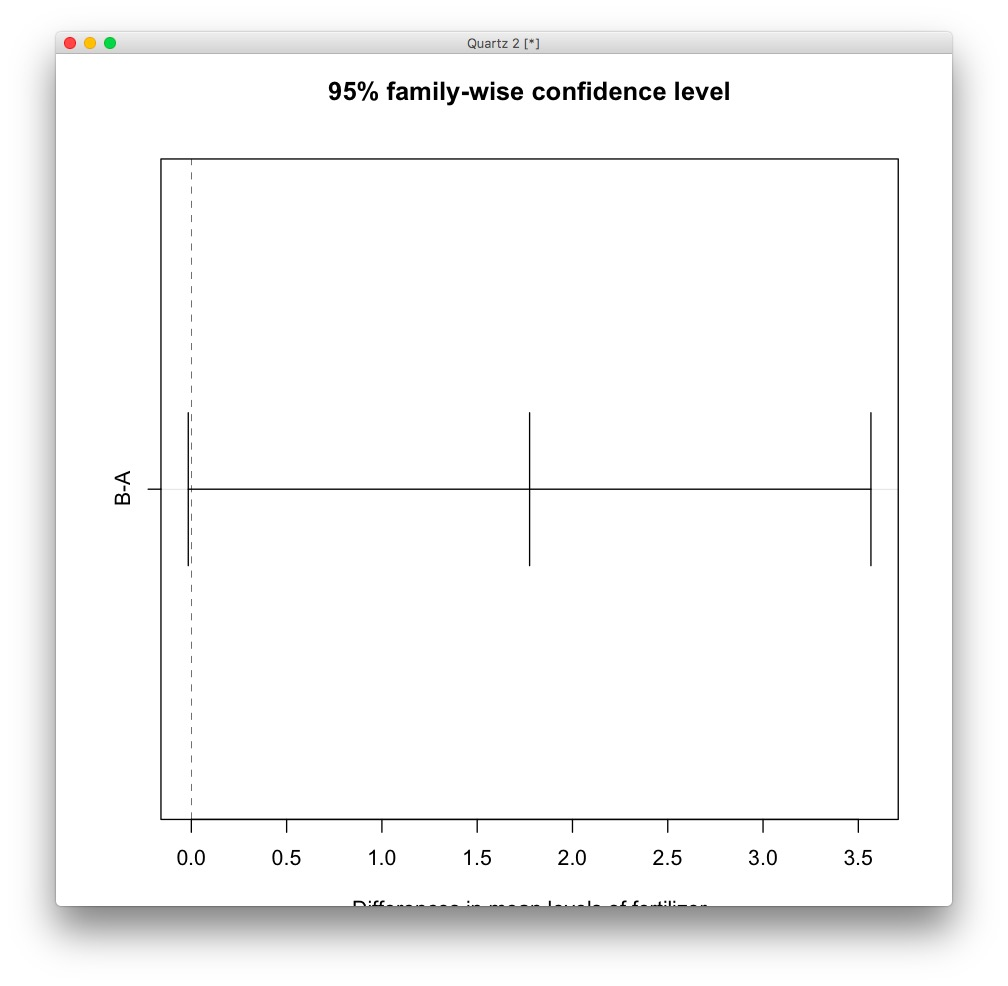
\includegraphics[width=\textwidth]{HW22.jpg}}
\end{center}

\begin{lstlisting}
          Tukey multiple comparisons of means
    95% family-wise confidence level

Fit: aov(formula = response ~ fertilizer)

fertilizer
     diff         lwr      upr     p adj
B-A 1.775 -0.01614443 3.566144 0.0519242
        \end{lstlisting}
Since the p-value is $0.0519242>\alpha=0.05$, we cannot reject that there's no difference between the two fertilizer types.\par

\bigbreak
\begin{addmargin}[-1.1em]{0em}
\textbf{(d)}\par\end{addmargin}
\end{addmargin}
\textbf{Test $H_0$ : No wheat effect against $H_1$ : there is a effect. Use $\alpha = 0.05$ if you reject $H_0$, use Tukey’s method to do pairwise comparisons of the different wheat types.}\par
    \bigbreak
    \begin{addmargin}[-0.5em]{0em}
    \textbf{Answer: }\end{addmargin}

According to the model we fit in (c), the p-value for wheat type is $4.59e-07<\alpha = 0.05$, so we reject the hypothesis that there's no wheat efffect.\par
 then we use the Tukey's method to do the pairwise comparisons of different wheat types:
\begin{lstlisting}
>fit <- aov(response~wheat)
>tk<-TukeyHSD(fit,"wheat")
>tk
>plot(tk)
\end{lstlisting}

\begin{lstlisting}
  Tukey multiple comparisons of means
    95% family-wise confidence level

Fit: aov(formula = response ~ wheat)

wheat
         diff        lwr       upr     p adj
"N"-"M"  4.30  2.4808709 6.1191291 0.0000107
"O"-"M"  5.15  3.3308709 6.9691291 0.0000008
"P"-"M"  3.50  1.6808709 5.3191291 0.0001557
"O"-"N"  0.85 -0.9691291 2.6691291 0.5687888
"P"-"N" -0.80 -2.6191291 1.0191291 0.6152451
"P"-"O" -1.65 -3.4691291 0.1691291 0.0839841
\end{lstlisting}

we get the following plot:

\begin{center} \makebox[\linewidth]{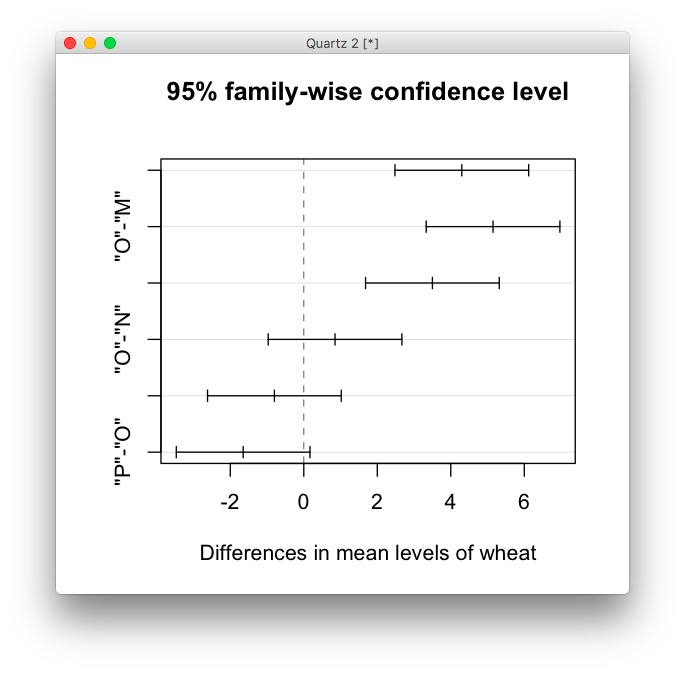
\includegraphics[width=\textwidth]{HW23.jpg}}
\end{center}

According to the plot and the p-value of the test, we arrive at a conclusion that there is no significant difference between wheat type P, N and O, but there is a significant difference between wheat type M and these three wheat types.



\end{document}

%Insert pics:
%%%%%%%%%%%%%
%\begin{center}
  %\makebox[\linewidth]{\includegraphics[width=\textwidth]{4640HW6.jpg}}
%\end{center}


%insert a complicated tab...
%%%%%%%%%%%%%%%%%%%%%%%%%%%%
%\begin{center}
%\begin{tabular}{ p{12cm}p{1cm}p{1cm}p{1cm}  }
%& \multicolumn{3}{c}{Posterior Quantiles} \\
%\centering{Quantity of Interest} & 25\% & 50\% & 75\% \\
%\hline
%geometric mean for Blue Earth (no basement), exp($\beta_2)$ &4.1& 5.0& 6.5\\
%geometric mean for Blue Earth County (basement), exp($\beta_1+\beta_2)$ &6.1 &7.1 &8.2\\
%geometric mean for Clay County (no basement), exp($\beta_3)$& 3.8& 4.7 &5.8\\
%geometric mean for Clay County (basement), exp($\beta_1+\beta_3)$ &5.6& 6.5& 7.6\\
%geometric mean for Goodhue County (no basement), exp($\beta_4)$ & 3.9 &4.9& 6.2\\
%geometric mean for Goodhue County (basement), exp($\beta_1+\beta_4)$ &5.8& 6.8& 7.9\\
%factor for basement vs. no basement, exp($\beta_1$)&1.1& 1.4 &1.7\\
%geometric sd of predictions, exp($\sigma$)&2.1 &2.2& 2.4\\
%\end{tabular}
%\end{center}


%%%insert code snippets:
%%%%%%%%%%%%%%%%%%%%%%%%
%\begin{lstlisting}
%INSERT CODE HERE
%\end{lstlisting}
